

%%%%%%%%%%%%%%%%%%%%%%%%%%%%%%%%%%%%%%%%%%%%%%%%%%%%%%%%%%%%%%%%%%%%%%%%%%%%%%%%%%%%%%%%%%%%%
\chapter{Generalizations, examples and connections}
This chapter is devoted for further discussions of Theorem \ref{thm:Demazure_operator_1}. Generalizations of Theorem \ref{thm:Demazure_operator_1} are discussed in Section \ref{sec:generalization}, while examples are shown by strands in Section \ref{sec:diagram}. Finally, we will mention about the connection between equivariant $K$-theory and equivariant cohomology in Section \ref{sec:AScompletion}. 

\section{Generalization}\label{sec:generalization}
In this section we generalize Theorem \ref{thm:Demazure_operator_1} in different directions. Quivers with loops are allowed, and the group actions can be replaced by $G \times \mathbb{C}^{\times}$-actions. After the generalization, we are able to cover the result in \cite[Theorem 7.2.5]{chriss1997representation}.

\subsection{Quiver with loops}
In this section we still assume the quiver has no cycles. For quiver with loops, we need to redefine Definition \ref{def:incidence_variety} in a strict version:
\begin{defn}[Incidence variety for strict flags]\label{def:incidence_variety_str}
For a quiver $Q$ with flag-type dimension vector $\ftdimvec{d}$, define
\begin{equation*}
\begin{aligned}
  \RRep_{\ftdimvec{d},\str}(Q):=\;& \left\{ (\rho,F) \in \Rep_{\dimvec{d}}(Q) \times \mathcal{F}_{\ftdimvec{d}}  \,\middle|\, \rho(M_j) \subseteq M_{j-1} \text{ for any } j \right\} \\
  \RRep_{\dimvec{d},\str}(Q):=\;& \left\{ (\rho,F) \in \Rep_{\dimvec{d}}(Q) \times \mathcal{F}_{\dimvec{d}}  \,\middle|\, \rho(M_j) \subseteq M_{j-1} \text{ for any } j \right\} \\
  =\;& \bigsqcup_{\ftdimvec{d}} \RRep_{\ftdimvec{d},\str}(Q)
\end{aligned}
\end{equation*}
and $\mu_{\ftdimvec{d},\str}$, $\pi_{\ftdimvec{d},\str}$, $\mu_{\dimvec{d},\str}$, $\pi_{\dimvec{d},\str}$ to be the natural morphisms from the incidence varieties to $\Rep_{\dimvec{d}}(Q)$ or flag varieties.
\end{defn}
We then replace $\RRep_{\dimvec{d}}(Q)$ by $\RRep_{\dimvec{d},\str}(Q)$. The Lie algebra $\mathfrak{r}_{\ww}$ (in Definition \ref{def:Lie_alg_with_rep}) is redefined by
\begin{equation*}
\begin{aligned}
  \mathfrak{r}_{\ww}:=\;& \left\{ (f_a)_{a\in Q_1} \in \Rep_{\dimvec{d}}(Q) \;\middle| \;  f_a(V_{\ww,j} \cap V_{s(a)}) \subseteq V_{\ww,j} \text{ for any } j \right\}\\
  \cong\;& \pi_{\dimvec{d},\str}^{-1}(\{F_{\ww} \})
\end{aligned}
\end{equation*}
then the same formula in Theorem \ref{thm:Demazure_operator_1} still works.
\subsection{$G \times \mathbb{C}^{\times}$-action}\label{subsec:Cstar_action}


The second generalization is about $G \times \mathbb{C}^{\times}$-actions. Recall the Remark \ref{rmk:action_on_flag}. Following the same arguments as in Example \ref{eg:K-initial-1}-\ref{eg:K-initial-4} and \ref{eg:H-initial-1}-\ref{eg:H-initial-4}, we get (in the Setting \ref{set:initial_case})
\begin{equation*}
\begin{aligned}
 &\Rpt(N \times \mathbb{C}^{\times}) \cong \Rpt(\mathbb{C}^{\times}) \cong \mathbb{Z}[q^{\pm 1 }]&&\Spt(N \times \mathbb{C}^{\times}) \cong \Spt(\mathbb{C}^{\times}) \cong \mathbb{Q}[t] \\
 &\Rpt(B \times \mathbb{C}^{\times}) \cong \Rpt(T \times \mathbb{C}^{\times}) \cong \mathbb{Z}[q^{\pm 1 }]\!\left[ e_1^{\pm 1},\ldots,e_n^{\pm 1} \right]&&\Spt(B \times \mathbb{C}^{\times}) \cong \Spt(T \times \mathbb{C}^{\times}) \cong \mathbb{Q}[t]\!\left[ \lambda_1,\ldots,\lambda_n \right]\\
 &\Rpt(G \times \mathbb{C}^{\times})  \cong \mathbb{Z}[q^{\pm 1}]\!\left[ e_1^{\pm 1},\ldots,e_n^{\pm 1} \right]^{S_n}&&\Spt(G \times \mathbb{C}^{\times}) \cong \mathbb{Q}[t]\!\left[ \lambda_1,\ldots,\lambda_n \right]^{S_n}\\ 
\end{aligned}
\end{equation*}

So everything remains the same except for the change of coefficient ring. In particular, for $D_i^{u,u'}:=[\St_{s_{i}}^{u,u'}]^{G_{\dimvec{d}} \times \mathbb{C}^{\times}}$, $f^{u}:=f \cdot \left[\RRep_{\ftdimvec{d},\str}(Q) \right]^{G_{\dimvec{d}}}$, we have formula \eqref{eq:final_destination}, with informations in Table \ref{table:euler_class_2}.

\begin{table}[ht]
  \vspace{0cm}
    \centering  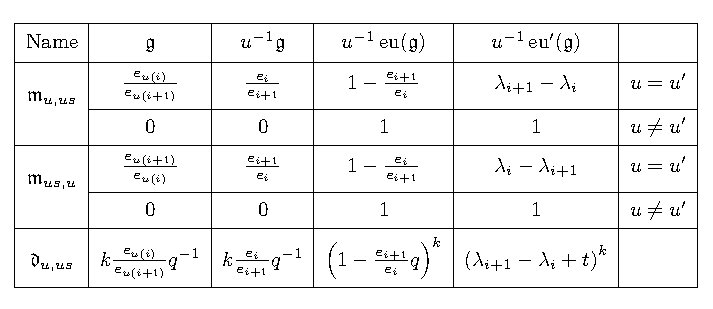
\includegraphics[width=12cm]{figures/table/table_euler_class_q.pdf}
      \caption{}
      \label{table:euler_class_2}        
\end{table}

\begin{theorem}\label{thm:Demazure_operator_2}
When the quiver has no cycle, we have a formula of Demazure operator for the $G_{\dimvec{d}} \times \mathbb{C}^{\times}$-action:
\begin{equation*}\label{eq:Demazure_operator_C*action}
D_i^{u,u'} \star f^{u'}=\begin{cases}
\left[\left( \raisebox{1mm}{$\displaystyle\frac{s_i f}{ 1-\frac{e_{i+1}}{e_{i}}}     + \frac{f}{1-\frac{e_{i}}{e_{i+1}}}$}  \right)\left(\displaystyle 1-\frac{e_{i+1}}{e_{i}} q\right)^{k} \right]^{u} & u=u',\\[8mm]
\left[s_i f  \left(\displaystyle 1-\frac{e_{i+1}}{e_{i}} q\right)^{k} \right]^{u} & u \neq u'.
\end{cases}
\end{equation*}
and similar for the equivariant cohomology theory:
\begin{equation*}\label{eq:Demazure_operator_cth_C*action}
\partial_i^{u,u'} \star f^{u'}=\begin{cases}
\left[\left( \displaystyle\frac{s_i f}{ \lambda_{i+1}-\lambda_{i}}     + \frac{f}{\lambda_{i}-\lambda_{i+1} }  \right)\left(\lambda_{i+1}-\lambda_{i} +t \right)^{k} \right]^{u} & u=u',\\[8mm]
\left[s_i f  \left(\lambda_{i+1}-\lambda_{i} +t\right)^{k} \right]^{u} & u \neq u'.
\end{cases}
\end{equation*}
\end{theorem}
%%%%%%%%%%%%%%%%%%%%%%%%%%%%%%%%%%%%%%%%%%%%%%%%%%%%%%%%%%%%%%%%%%%%%%%%%%%%%%%%%%%%%%%%%%%%%
\section{From formula to diagram}\label{sec:diagram}
This section is designed for showing examples. Recall Proposition \ref{prop:5-case-0.05} that every $\ftdimvec{d}$ or $u$ corresponds to an ordered set of colored points. It can be imagined that the lines connecting two ordered sets represents one element in $K^{G_{\dimvec{d}}}(\St_{\dimvec{d}})$. Actually, we draw the picture of generators of $K^{G_{\dimvec{d}}}(\St_{\dimvec{d}})$ in Figure \ref{fig:generators}, where
$$e_{i}^{u}=:e_{u^{-1}(i)} \left[ \RRep_{u}(Q) \right]^{G_{\dimvec{d}}} \in K^{G_{\dimvec{d}}} \left( \RRep_{u}(Q) \right) \hookrightarrow K^{G_{\dimvec{d}}} \left( \St^{u,u} \right).$$

\begin{figure}[ht]
  \vspace{0cm}
    \centering  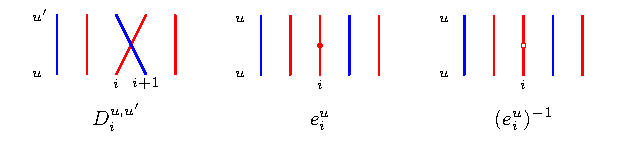
\includegraphics[width=12cm]{figures/strands/generators.pdf}
      \caption{}
      \label{fig:generators}        
\end{figure}

The convolution product can be then viewed as pictures gluing vertically, where the incompatibility of colors gives $0$. For example,

\begin{figure}[ht]
  \vspace{0cm}
    \centering  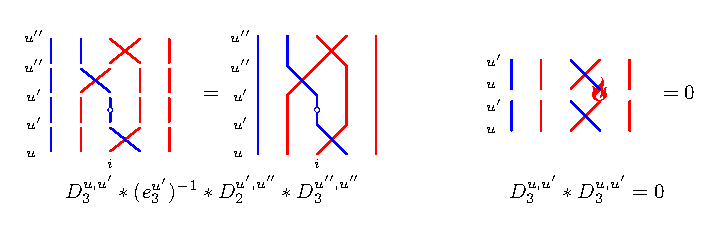
\includegraphics[width=12cm]{figures/strands/glue_vertically.pdf}
      \label{fig:glue_vertically}        
\end{figure}

By Proposition \ref{prop:generators}, every element in $K^{G_{\dimvec{d}}}(\St_{\dimvec{d}})= \oplus_{u,u'} K^{G_{\dimvec{d}}}(\St^{u,u'})$  can be expressed as a $\mathbb{Z}$-linear combination of strands. The expressions are not unique, so we need to find out their relations. Some relations are clear from the picture (but still need to check), for example,

\begin{figure}[ht]
  \vspace{0cm}
    \centering  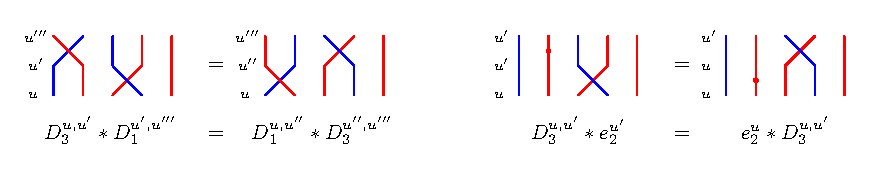
\includegraphics[width=15cm]{figures/strands/clear_relations.pdf}
      \label{fig:clear_relations}        
\end{figure}

We won't draw these ``obvious" relations later. The first nontrivial relation comes from the following lemma.

\begin{lemma}\label{lem:convolution_product_1}
For $f \in \Rpt(T_{\dimvec{d}})$, denote $D_i^{u,u'} =\left[\St_{s_{i}}^{u,u'}\right]^{G_{\dimvec{d}}}$, $f^{u}=f \cdot \left[ \RRep_{\dimvec{d}}(Q) \right]^{G_{\dimvec{d}}} \in K^{G_{\dimvec{d}}} (\St_{\dimvec{d}})$, we have
$$D_i^{u,u'} \fakestar f^{u'}= (s_i f)^{u} \fakestar D_i^{u,u'} +  \delta_{u,u'}\left[\left(s_i f-f\right) \frac{e_{i+1}}{e_i}  \left(\displaystyle 1-\frac{e_{i+1}}{e_{i}}\right)^{k-1} \right]^{u}.$$
Similarly, for the $G_{\dimvec{d}}$-equivariant cohomology theory, we have
$$\partial_i^{u,u'} \fakestar f^{u'}= (s_i f)^{u} \fakestar \partial_i^{u,u'} +  \delta_{u,u'}\left[\left(s_i f-f\right)   \left(\lambda_{i+1}-\lambda_{i}\right)^{k-1} \right]^{u}.$$
In the formula, $k$ stands for the number of arrows from the vertex associated to $v_{u(i+1)}$ to the vertex associated to $v_{u(i)}$.
\end{lemma}
\begin{proof}
By Proposition \ref{prop:generators}, we only need to show, for any $g \in \Rpt(T_{\dimvec{d}})$,
$$D_i^{u,u'} \fakestar f^{u'} \star g^{u'}= (s_i f)^{u} \fakestar D_i^{u,u'} \star g^{u'} +  \delta_{u,u'}\left[\left(s_i f-f\right) \frac{e_{i+1}}{e_i}  \left(\displaystyle 1-\frac{e_{i+1}}{e_{i}}\right)^{k-1} \right]^{u} \star g^{u'}.$$
Now we apply Theorem \ref{thm:Demazure_operator_1}. The same argument works for equivariant cohomology theory.
\end{proof}
Lemma \ref{lem:convolution_product_1} explains ``what happens when a point walk through a crossing". The convolution algebra $H_{G_{\dimvec{d}}}^{*}(\St_{\dimvec{d}})$ is called the \textbf{KLR-algebra}. The relations of the KLR-algebra can be found in \cite[Definition 3.2.2]{seiffarth2017klr}, and we will only show the relations of $K$-theoretical version.
\begin{warning}
In the following examples, $\fakestar$ is often omitted for simplicity.
\end{warning}
\subsection{One point quiver}
We begin with the trivial quiver, which has only one vertex and no arrows. Everything is simplified: 
$$\WWd=\Wd,\quad \MinWd =\{\Id \}, \quad \RRep_{\dimvec{d}}(Q) \cong \mathcal{F}_{\dimvec{d}}, \quad \St_{\dimvec{d}} \cong\mathcal{F}_{\dimvec{d}} \times \mathcal{F}_{\dimvec{d}},$$
$$K^{G_{\dimvec{d}}} (\mathcal{F}_{\dimvec{d}}) \cong \mathbb{Z}\!\left[ e_1^{\pm 1},\ldots,e_{\abdimvec{d}}^{\pm 1} \right], \qquad H_{G_{\dimvec{d}}}^{*}(\mathcal{F}_{\dimvec{d}}) \cong \mathbb{Q}[\lambda_1,\ldots,\lambda_{\abdimvec{d}}].$$
In this case, $K^{G_{\dimvec{d}}} (\mathcal{F}_{\dimvec{d}} \times  \mathcal{F}_{\dimvec{d}})$ is called the \textbf{$\boldsymbol{K}$-theoretic NilHecke algebra}, and $H_{G_{\dimvec{d}}}^{*}(\mathcal{F}_{\dimvec{d}} \times  \mathcal{F}_{\dimvec{d}})$ is called the \textbf{(cohomological) NilHecke algebra}.

The formulas in Theorem \ref{thm:Demazure_operator_1} and Lemma \ref{lem:convolution_product_1} are simplified: (superscripts are omitted, and functions $f$ in four formulas lie in $K^{G_{\dimvec{d}}} (\mathcal{F}_{\dimvec{d}})$, $K^{G_{\dimvec{d}}} (\mathcal{F}_{\dimvec{d}} \times  \mathcal{F}_{\dimvec{d}})$, $H_{G_{\dimvec{d}}}^{*}(\mathcal{F}_{\dimvec{d}})$ and $H_{G_{\dimvec{d}}}^{*}(\mathcal{F}_{\dimvec{d}} \times  \mathcal{F}_{\dimvec{d}})$, respectively)
\begin{equation*}
\begin{aligned}
  D_i \star f =\;& \frac{s_i f}{1- \frac{e_{i+1}}{e_i}} + \frac{f}{1- \frac{e_{i}}{e_{i+1}}}\\ 
  \partial_i \star f =\;& \frac{s_i f}{\lambda_{i+1}-\lambda_{i}}+\frac{ f}{\lambda_{i}-\lambda_{i+1}}=\frac{f -s_i f}{\lambda_{i}-\lambda_{i+1}}\\
  D_i f =\;& (s_i f) D_i + \frac{f- s_i f}{1- \frac{e_{i}}{e_{i+1}}}\\ 
  \partial_i f =\;& (s_i f) \partial_i + \frac{f- s_i f}{\lambda_{i}-\lambda_{i+1}}\\   
\end{aligned}
\end{equation*}

The relations for $D_i$ are shown in Figure \ref{fig:relations_1}.
\begin{figure}[ht]
  \vspace{0cm}
    \centering 
    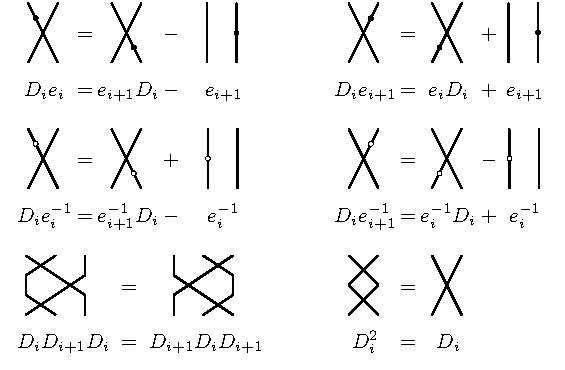
\includegraphics[width=10cm]{figures/strands/relations_1.pdf} 
    \caption{}
      \label{fig:relations_1}        
\end{figure}
\subsection{$A_2$-quiver}
Now let us consider the $A_2$-quiver $\begin{tikzcd}[ampersand replacement=\&]
	\textcolor{red}{\bullet} \& \textcolor{blue}{\bullet} 
	\arrow[from=1-1, to=1-2]
 \end{tikzcd}$. This time we have to color the dots and strands. In this case,
$$K^{G_{\dimvec{d}}} \left(\RRep_{\dimvec{d}}(Q)\right) \cong \bigoplus_{u} \mathbb{Z}\!\left[ e_1^{u,\pm 1},\ldots,e_{\abdimvec{d}}^{u,\pm 1} \right], \qquad H_{G_{\dimvec{d}}}^{*}\!\!\left(\RRep_{\dimvec{d}}(Q)\right) \cong \bigoplus_{u} \mathbb{Q}\left[\lambda_1^{u},\ldots,\lambda_{\abdimvec{d}}^{u}\right].$$
The formulas in Theorem \ref{thm:Demazure_operator_1} and Lemma \ref{lem:convolution_product_1} are simplified: 
\begingroup
\allowdisplaybreaks
\begin{align*}
  D_i^{u,u'} \star f^{u'}=\;&\begin{cases}
  \left[ \raisebox{1mm}{$\displaystyle\frac{s_i f}{ 1-\frac{e_{i+1}}{e_{i}}}     + \frac{f}{1-\frac{e_{i}}{e_{i+1}}}$}   \right]^{u} & \text{\small\raisebox{-0.5mm}{\ding{192}}}\begin{tikzcd}[ampersand replacement=\&]
    	u=u'
     \end{tikzcd},\\[4mm]
  \left[s_i f  \left(\displaystyle 1-\frac{e_{i+1}}{e_{i}}\right) \right]^{u} & \text{\small\raisebox{-0.5mm}{\ding{193}}}\begin{tikzcd}[ampersand replacement=\&]
  	\textcolor{red}{u(i+1)} \& \textcolor{blue}{u(i)} 
  	\arrow[from=1-1, to=1-2]
   \end{tikzcd},\\[3mm]
  \left(s_i f \right)^{u} & \text{\small\raisebox{-0.5mm}{\ding{194}}}\begin{tikzcd}[ampersand replacement=\&]
    	\textcolor{red}{u(i)} \& \textcolor{blue}{u(i+1)} 
    	\arrow[from=1-1, to=1-2]
     \end{tikzcd}.\\
  \end{cases}\\ 
  \partial_i^{u,u'} \star f^{u'}=\;&\begin{cases}
  \left[\displaystyle\frac{f - s_i f}{ \lambda_i-\lambda_{i+1}}  \right]^{u} \hspace{16mm}$\,$& \text{\small\raisebox{-0.5mm}{\ding{192}}}\begin{tikzcd}[ampersand replacement=\&]
      	u=u'
       \end{tikzcd},\\[3mm]
  \left[s_i f  \left(\lambda_{i+1}-\lambda_i\right) \right]^{u} & \text{\small\raisebox{-0.5mm}{\ding{193}}}\begin{tikzcd}[ampersand replacement=\&]
  	\textcolor{red}{u(i+1)} \& \textcolor{blue}{u(i)} 
  	\arrow[from=1-1, to=1-2]
   \end{tikzcd},\\[3mm]
  \left(s_i f \right)^{u} &\text{\small\raisebox{-0.5mm}{\ding{194}}} \begin{tikzcd}[ampersand replacement=\&]
    	\textcolor{red}{u(i)} \& \textcolor{blue}{u(i+1)} 
    	\arrow[from=1-1, to=1-2]
     \end{tikzcd}.\\
  \end{cases}\\ 
  D_i^{u,u'} f^{u'} =\;& (s_i f)^{u} D_i^{u,u'} + \left[\frac{f- s_i f}{1- \frac{e_{i}}{e_{i+1}}}\right]^{u}\\ 
  \partial_i^{u,u'} f^{u'} =\;& (s_i f)^{u} \partial_i^{u,u'} + \left[\frac{f- s_i f}{\lambda_{i}-\lambda_{i+1}}\right]^{u}\\   
\end{align*}
\endgroup

Part of relations for $D_i$ are shown in Figure \ref{fig:relations_2}.
\begin{figure}[ht]
  \vspace{0cm}
    \centering  
    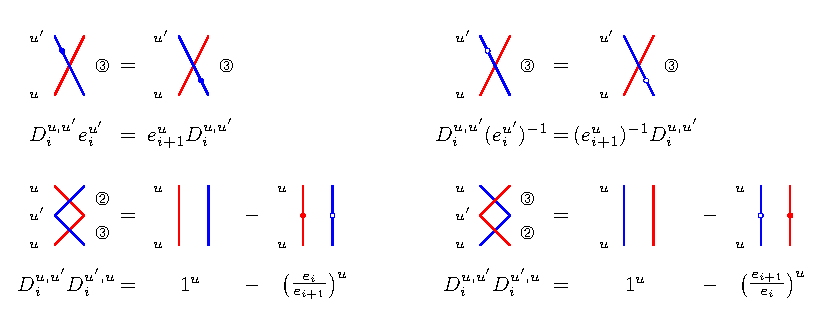
\includegraphics[width=13cm]{figures/strands/relations_2.pdf} 
    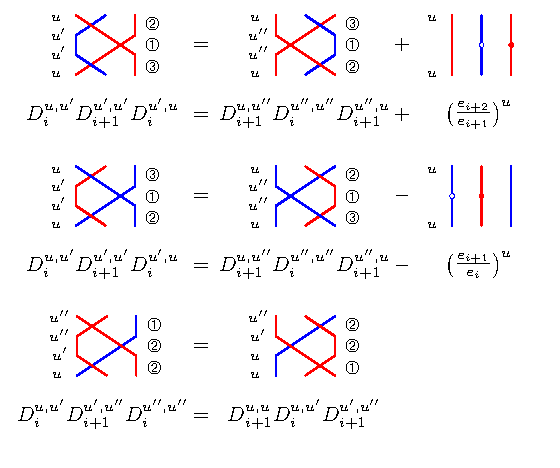
\includegraphics[width=10cm]{figures/strands/relations_3.pdf} 
    \caption{}
      \label{fig:relations_2}        
\end{figure}
\subsection{$1$-loop quiver}
In this subsection we try to give a simplest example for Section \ref{sec:generalization}, which is the $1$-loop quiver. In this case,
$$K^{G_{\dimvec{d}}} \left(\RRep_{\dimvec{d},\str}(Q)\right) \cong  \mathbb{Z}\!\left[ e_1^{\pm 1},\ldots,e_{\abdimvec{d}}^{\pm 1} \right], \qquad H_{G_{\dimvec{d}}}^{*}\!\!\left(\RRep_{\dimvec{d},\str}(Q)\right) \cong  \mathbb{Q}\left[\lambda_1,\ldots,\lambda_{\abdimvec{d}}\right].$$
The formulas in Theorem \ref{thm:Demazure_operator_1} and Lemma \ref{lem:convolution_product_1} are simplified:

\begin{equation*}
\begin{aligned}
  D_i \star f =\;& s_i f + f\cdot \frac{e_{i+1}}{e_{i}}\\ 
  \partial_i \star f =\;& f -s_i f\\
  D_i f =\;& (s_i f) D_i + (s_i f-f) \frac{e_{i+1}}{e_i}\\ 
  \partial_i f =\;& (s_i f) \partial_i + (s_i f-f)\\   
\end{aligned}
\end{equation*}

Now for the $G_{\dimvec{d}} \times \mathbb{C}^{\times}$-action. We have analog of Lemma \ref{lem:convolution_product_1} for $G_{\dimvec{d}} \times \mathbb{C}^{\times}$-action:
\begin{lemma}\label{lem:convolution_product_2}
For $f \in \Rpt(T_{\dimvec{d}} \times \mathbb{C}^{\times})$, denote $D_i^{u,u'} =\left[\St_{s_{i}}^{u,u'}\right]^{G_{\dimvec{d}}\times \mathbb{C}^{\times}}$, $f^{u}=f \cdot \left[ \RRep_{\dimvec{d}}(Q) \right]^{G_{\dimvec{d}}\times \mathbb{C}^{\times}} \in K^{G_{\dimvec{d}}\times \mathbb{C}^{\times}} (\St_{\dimvec{d}})$, we have
$$D_i^{u,u'} \fakestar f^{u'}= (s_i f)^{u} \fakestar D_i^{u,u'} +  \delta_{u,u'}\left[\left(f-s_i f\right) \raisebox{-1mm}{$\displaystyle\frac{\left( 1-\frac{e_{i+1}}{e_{i}} q\right)^{k}}{ 1-\frac{e_{i}}{e_{i+1}}}$}\right]^{u}.$$
Similarly, for the $(G_{\dimvec{d}}\times \mathbb{C}^{\times})$-equivariant cohomology theory, we have
$$\partial_i^{u,u'} \fakestar f^{u'}= (s_i f)^{u} \fakestar \partial_i^{u,u'} +  \delta_{u,u'}\left[\left(f-s_i f\right) 
\frac{\left(\lambda_{i+1}-\lambda_{i}+t\right)^{k}}{\lambda_{i}-\lambda_{i+1}}   \right]^{u}.$$
In the formula, $k$ stands for the number of arrows from the vertex associated to $v_{u(i+1)}$ to the vertex associated to $v_{u(i)}$.
\end{lemma}
In the $1$-loop quiver case, notice that
$$K^{G_{\dimvec{d}} \times \mathbb{C}^{\times}} \left(\RRep_{\dimvec{d},\str}(Q)\right) \cong  \mathbb{Z}\left[q^{\pm 1}\right]\!\left[ e_1^{\pm 1},\ldots,e_{\abdimvec{d}}^{\pm 1} \right], \quad H_{G_{\dimvec{d}}\times \mathbb{C}^{\times}}^{*}\!\!\left(\RRep_{\dimvec{d},\str}(Q)\right) \cong  \mathbb{Q}[t]\left[\lambda_1,\ldots,\lambda_{\abdimvec{d}}\right].$$

The formulas in Theorem \ref{thm:Demazure_operator_2} and Lemma \ref{lem:convolution_product_2} are simplified:

\begin{equation*}
\begin{aligned}
  D_i \star f=\;&
  \left( \raisebox{1mm}{$\displaystyle\frac{s_i f}{ 1-\frac{e_{i+1}}{e_{i}}}     + \frac{f}{1-\frac{e_{i}}{e_{i+1}}}$}  \right)\left(\displaystyle 1-\frac{e_{i+1}}{e_{i}} q\right)^{k} \\
  \partial_i \star f =\;& (f -s_i f) \frac{\lambda_{i+1}-\lambda_{i}+t}{\lambda_{i}-\lambda_{i+1}}\\
  D_i f =\;& (s_i f) D_i + \left(f-s_i f\right) \displaystyle\frac{ 1-\frac{e_{i+1}}{e_{i}} q}{ 1-\frac{e_{i}}{e_{i+1}}}\\ 
  \partial_i f =\;& (s_i f) \partial_i + (f-s_i f) \frac{\lambda_{i+1}-\lambda_{i}+t}{\lambda_{i}-\lambda_{i+1}}\\   
\end{aligned}
\end{equation*}
Readers are welcomed to write a complete set of relations.
%??? Center of the algebra can be also computed
%%%%%%%%%%%%%%%%%%%%%%%%%%%%%%%%%%%%%%%%%%%%%%%%%%%%%%%%%%%%%%%%%%%%%%%%%%%%%%%%%%%%%%%%%%%%%
\section{Atiyah--Segal completion theorem}\label{sec:AScompletion}

Different cohomology theories are connected in a incredible way. In this section, we describe the Atiyah--Segal completion theorem, which connect $G$-equivariant $K$-theory with $G$-equivariant cohomology theory. Roughly speaking, they are isomorphic after completion (and base change to $\mathbb{Q}$).

For an algebraic group $G$, denote
$$I:= \ker \left(\Rpt(G) \longrightarrow \Rpt(\Id) \right) \qquad J:= \ker \left(\Spt(G) \longrightarrow \Spt(\Id) \right)$$
as the augmentation ideals in $\Rpt(G)$ and $\Spt(G)$, respectively. We denote
$$K^G(X)_I^{\wedge}:= \varprojlim_n K^G(X)/\left(I^n K^G(X) \right) \qquad H_G^{*}(X)_J^{\wedge}:= \varprojlim_n H_G^{*}(X)/\left(J^n H_G^{*}(X) \right)$$
as the $I$-adic (resp. $J$-adic) completion.

\begin{theorem}[Atiyah--Segal completion theorem]\label{thm:Atiyah--Segal_completion_theorem}
For a $G$-variety $X$, the Atiyah--Segal map from the equivariant $K$-theory to the ordinary topological $K$-theory
$$\AS:K^G(X)_I^{\wedge} \longrightarrow K(\EGG G \times^G X ) $$
is an isomorphism, and the (cohomology) Chern class map (defined in \cite[5.8]{chriss1997representation})
$$\chern: K(\EGG G \times^G X ) \longrightarrow H_G^{*}(X)_J^{\wedge}$$
is an isomorphism after base change to $\mathbb{Q}$.
\end{theorem}

Instead of explaining terminologies in Theorem \ref{thm:Atiyah--Segal_completion_theorem}, let us see some examples and get a feeling how that works.

\begin{eg}
For $G=\mathbb{C}^{\times}$,
$$\Rpt(\mathbb{C}^{\times}) \cong \mathbb{Z}\!\left[e^{\pm 1} \right], I=(e-1), \quad \Spt(\mathbb{C}^{\times}) \cong \mathbb{Q}\!\left[\lambda \right], J=(\lambda), $$
we get the following diagram:
% https://q.uiver.app/?q=WzAsMTIsWzEsMCwiS157XFxtYXRoYmJ7Q31ee1xcdGltZXN9fVxcIShcXHB0KV9JXntcXHdlZGdlfSJdLFsyLDAsIksoXFxCR0cgXFxtYXRoYmJ7Q31ee1xcdGltZXN9KSJdLFszLDAsIkhfe1xcbWF0aGJie0N9XntcXHRpbWVzfX1eeyp9XFwhKFxccHQpX0pee1xcd2VkZ2V9Il0sWzAsMCwiS157XFxtYXRoYmJ7Q31ee1xcdGltZXN9fVxcIShcXHB0KSJdLFs0LDAsIkhfe1xcbWF0aGJie0N9XntcXHRpbWVzfX1eeyp9XFwhKFxccHQpIl0sWzAsMSwiXFxtYXRoYmJ7Wn1cXCFcXGxlZnRbZV57XFxwbSAxfSBcXHJpZ2h0XSJdLFsxLDEsIlxcbWF0aGJie1p9XFwhXFxsZWZ0W1xcbGVmdFtlLTFcXHJpZ2h0XSBcXHJpZ2h0XSJdLFsyLDEsIlxcbWF0aGJie1p9XFwhXFxsZWZ0W1xcbGVmdFtlLTFcXHJpZ2h0XSBcXHJpZ2h0XSJdLFszLDEsIlxcbWF0aGJie1F9XFwhXFxsZWZ0W1xcbGVmdFtcXGxhbWJkYVxccmlnaHRdIFxccmlnaHRdIl0sWzQsMSwiXFxtYXRoYmJ7UX1cXCFcXGxlZnRbXFxsYW1iZGEgXFxyaWdodF0iXSxbMiwyLCJlLTEiXSxbMywyLCJlXntcXGxhbWJkYX0tMSJdLFswLDEsIlxcQVMiXSxbMSwyLCJcXGNoZXJuIl0sWzYsN10sWzcsOF0sWzMsMCwiXFxzdWJzZXRlcSIsMSx7InN0eWxlIjp7ImJvZHkiOnsibmFtZSI6Im5vbmUifSwiaGVhZCI6eyJuYW1lIjoibm9uZSJ9fX1dLFs1LDYsIlxcc3Vic2V0ZXEiLDEseyJzdHlsZSI6eyJib2R5Ijp7Im5hbWUiOiJub25lIn0sImhlYWQiOnsibmFtZSI6Im5vbmUifX19XSxbNCwyLCJcXHN1cHNldGVxIiwxLHsic3R5bGUiOnsiYm9keSI6eyJuYW1lIjoibm9uZSJ9LCJoZWFkIjp7Im5hbWUiOiJub25lIn19fV0sWzksOCwiXFxzdXBzZXRlcSIsMSx7InN0eWxlIjp7ImJvZHkiOnsibmFtZSI6Im5vbmUifSwiaGVhZCI6eyJuYW1lIjoibm9uZSJ9fX1dLFsxMCwxMSwiIiwwLHsic3R5bGUiOnsidGFpbCI6eyJuYW1lIjoibWFwcyB0byJ9fX1dXQ==
\[\begin{tikzcd}[column sep={between origins, 30mm}, row sep={between origins, 7mm}]
	{K^{\mathbb{C}^{\times}}\!(\pt)} &[-10mm] {K^{\mathbb{C}^{\times}}\!(\pt)_I^{\wedge}} & {K(\BGG \mathbb{C}^{\times})} & {H_{\mathbb{C}^{\times}}^{*}\!(\pt)_J^{\wedge}} &[-10mm] {H_{\mathbb{C}^{\times}}^{*}\!(\pt)} \\
	{\mathbb{Z}\!\left[e^{\pm 1} \right]} & {\mathbb{Z}\!\left[\left[e-1\right] \right]} & {\mathbb{Z}\!\left[\left[e-1\right] \right]} & {\mathbb{Q}\!\left[\left[\lambda\right] \right]} & {\mathbb{Q}\!\left[\lambda \right]} \\
	&& {e-1} & {e^{\lambda}-1}
	\arrow["\AS", from=1-2, to=1-3]
	\arrow["\chern", from=1-3, to=1-4]
	\arrow[from=2-2, to=2-3]
	\arrow[from=2-3, to=2-4]
	\arrow["\subseteq"{description}, draw=none, from=1-1, to=1-2]
	\arrow["\subseteq"{description}, draw=none, from=2-1, to=2-2]
	\arrow["\supseteq"{description}, draw=none, from=1-5, to=1-4]
	\arrow["\supseteq"{description}, draw=none, from=2-5, to=2-4]
	\arrow[maps to, from=3-3, to=3-4]
\end{tikzcd}\]
This can be generalized to any torus $T$ of rank $n$.
\end{eg}

\begin{eg}\label{eg:AS_initial}
For $G=\GL_n$, $X=\mathcal{F}$,
\begin{equation*}
\begin{aligned}
   \Rpt(\GL_n) \cong\;& \mathbb{Z}\!\left[ e_1^{\pm 1},\ldots,e_n^{\pm 1} \right]^{S_n}, &&I'=\left\{ f \in \Rpt(\GL_n)  \;\middle|\;\rule{0mm}{3.6mm} f(1,\ldots, 1)=0 \right\}\\ 
  \Spt(\GL_n) \cong\;&  \mathbb{Q}\!\left[ \lambda_1,\ldots,\lambda_n \right]^{S_n},&&J'=\left\{ f \in \Spt(\GL_n)  \;\middle|\;\rule{0mm}{3.6mm} f(0,\ldots, 0)=0 \right\}.
\end{aligned}
\end{equation*}
We have the commutative diagram
% https://q.uiver.app/?q=WzAsMTAsWzEsMCwiS157XFxHTF9ufSAoXFxtYXRoY2Fse0Z9KV97SSd9XntcXHdlZGdlfSJdLFsyLDAsIksoXFxFR0cgR0xfbiBcXHRpbWVzXntcXEdMX259XFxtYXRoY2Fse0Z9KSJdLFszLDAsIkhfe0dMX259XnsqfVxcIShcXG1hdGhjYWx7Rn0pX3tKJ31ee1xcd2VkZ2V9Il0sWzAsMCwiS157XFxHTF9ufSAoXFxtYXRoY2Fse0Z9KSJdLFs0LDAsIkhfe0dMX259XnsqfVxcIShcXG1hdGhjYWx7Rn0pIl0sWzAsMSwiS157VH0gKFxccHQpIl0sWzEsMSwiS157VH0gKFxccHQpX3tJfV57XFx3ZWRnZX0iXSxbMiwxLCJLKEJUKSJdLFszLDEsIkhfe1R9XnsqfVxcIShcXHB0KV97Sn1ee1xcd2VkZ2V9Il0sWzQsMSwiSF97VH1eeyp9XFwhKFxccHQpIl0sWzAsMSwiXFxBUyJdLFsxLDIsIlxcY2hlcm4iXSxbNiw3LCJcXEFTIl0sWzcsOCwiXFxjaGVybiJdLFszLDAsIlxcc3Vic2V0ZXEiLDEseyJzdHlsZSI6eyJib2R5Ijp7Im5hbWUiOiJub25lIn0sImhlYWQiOnsibmFtZSI6Im5vbmUifX19XSxbNSw2LCJcXHN1YnNldGVxIiwxLHsic3R5bGUiOnsiYm9keSI6eyJuYW1lIjoibm9uZSJ9LCJoZWFkIjp7Im5hbWUiOiJub25lIn19fV0sWzQsMiwiXFxzdXBzZXRlcSIsMSx7InN0eWxlIjp7ImJvZHkiOnsibmFtZSI6Im5vbmUifSwiaGVhZCI6eyJuYW1lIjoibm9uZSJ9fX1dLFs5LDgsIlxcc3Vwc2V0ZXEiLDEseyJzdHlsZSI6eyJib2R5Ijp7Im5hbWUiOiJub25lIn0sImhlYWQiOnsibmFtZSI6Im5vbmUifX19XSxbNCw5XSxbMiw4XSxbMSw3XSxbMCw2XSxbMyw1XV0=
\[\begin{tikzcd}[
  row sep=small,column sep={between origins, 40mm},
  ar symbol/.style = {draw=none,"\textstyle#1" description,sloped},
  isomorphic/.style = {ar symbol={\cong}},
  ]
	{K^{\GL_n} (\mathcal{F})} &[-20mm] {K^{\GL_n} (\mathcal{F})_{I'}^{\wedge}} & {K\left(\EGG GL_n \times^{\GL_n}\mathcal{F}\right)} & {H_{GL_n}^{*}\!(\mathcal{F})_{J'}^{\wedge}} &[-20mm] {H_{GL_n}^{*}\!(\mathcal{F})} \\
	{K^{T} (\pt)} & {K^{T} (\pt)_{I}^{\wedge}} & {K(BT)} & {H_{T}^{*}\!(\pt)_{J}^{\wedge}} & {H_{T}^{*}\!(\pt)}
	\arrow["\AS", from=1-2, to=1-3]
	\arrow["\chern", from=1-3, to=1-4]
	\arrow["\AS", from=2-2, to=2-3]
	\arrow["\chern", from=2-3, to=2-4]
	\arrow["\subseteq"{description}, draw=none, from=1-1, to=1-2]
	\arrow["\subseteq"{description}, draw=none, from=2-1, to=2-2]
	\arrow["\supseteq"{description}, draw=none, from=1-5, to=1-4]
	\arrow["\supseteq"{description}, draw=none, from=2-5, to=2-4]
	\arrow[from=1-5, to=2-5, isomorphic]
	\arrow[from=1-4, to=2-4, isomorphic]
	\arrow[from=1-3, to=2-3, isomorphic]
	\arrow[from=1-2, to=2-2, isomorphic]
	\arrow[from=1-1, to=2-1, isomorphic]
\end{tikzcd}\]
which reduce to Example \ref{eg:AS_initial}.

Under this isomorphism, the Demazure operator $D_i$ is sent to $\partial_i \fakestar \displaystyle\frac{\lambda_{i}-\lambda_{i+1}}{1-\exp(\lambda_{i}-\lambda_{i+1})}$, i.e., the diagram \eqref{eq:Todd_class} commutes:
% https://q.uiver.app/?q=WzAsNCxbMCwwLCJLXntcXEdMX259IChcXG1hdGhjYWx7Rn0pX3tJJ31ee1xcd2VkZ2V9IFxcb3RpbWVzX3tcXG1hdGhiYntafX1cXG1hdGhiYntRfSJdLFsyLDAsIkhfe0dMX259XnsqfVxcIShcXG1hdGhjYWx7Rn0pX3tKJ31ee1xcd2VkZ2V9Il0sWzAsMSwiS157XFxHTF9ufSAoXFxtYXRoY2Fse0Z9KV97SSd9XntcXHdlZGdlfSBcXG90aW1lc197XFxtYXRoYmJ7Wn19XFxtYXRoYmJ7UX0iXSxbMiwxLCJIX3tHTF9ufV57Kn1cXCEoXFxtYXRoY2Fse0Z9KV97Sid9XntcXHdlZGdlfSJdLFsxLDMsIlxccGFydGlhbF9pIFxcZmFrZXN0YXIgXFxmcmFje1xcbGFtYmRhX3tpfS1cXGxhbWJkYV97aSsxfX17MS1lXntcXGxhbWJkYV97aX0tXFxsYW1iZGFfe2krMX19fSJdLFswLDIsIkRfaSIsMl0sWzAsMSwiXFxjaGVybiBcXGNpcmMgXFxBUyJdLFsyLDMsIlxcY2hlcm4gXFxjaXJjIFxcQVMiXV0=
\begin{equation}\label{eq:Todd_class}
\begin{tikzcd}[column sep=large]
	{K^{\GL_n} (\mathcal{F})_{I'}^{\wedge} \otimes_{\mathbb{Z}}\mathbb{Q}} && {H_{GL_n}^{*}\!(\mathcal{F})_{J'}^{\wedge}} \\
	{K^{\GL_n} (\mathcal{F})_{I'}^{\wedge} \otimes_{\mathbb{Z}}\mathbb{Q}} && {H_{GL_n}^{*}\!(\mathcal{F})_{J'}^{\wedge}}
	\arrow["{\partial_i \fakestar \frac{\lambda_{i}-\lambda_{i+1}}{1-e^{\lambda_{i}-\lambda_{i+1}}}}", from=1-3, to=2-3]
	\arrow["{D_i}"', from=1-1, to=2-1]
	\arrow["{\chern \circ \AS}", from=1-1, to=1-3]
	\arrow["{\chern \circ \AS}", from=2-1, to=2-3]
\end{tikzcd}
\end{equation}
\end{eg}

As a quotient of two (different types of) Euler class, the \textbf{Todd class}
$$\Td_i:=\frac{\lambda_{i}-\lambda_{i+1}}{1-e^{\lambda_{i}-\lambda_{i+1}}}$$
measures the noncommutativity of \eqref{eq:Todd_class} when $\partial_i \fakestar \displaystyle\frac{\lambda_{i}-\lambda_{i+1}}{1-\exp(\lambda_{i}-\lambda_{i+1})}$ is replaced by $\partial_i$.